\documentclass{article}
\usepackage{graphicx}
\usepackage{amsmath}
\usepackage{tikz}
\usepackage{tikz-layers}
\usetikzlibrary{calc, shapes, positioning}
\usepackage{bbm}
\usepackage{natbib}
\usepackage[margin=1in]{geometry}
\usepackage{caption}
\usepackage{booktabs}
\usepackage{subcaption}

\title{BIOS 735 Project Report}
\author{Abby Foes, Zheng Lan, Justin Landis, Yu Liu, Alec Reinhardt}
\date{April 2025}

\begin{document}

\maketitle

\section{Introduction}

\subsection*{Data Description}

\noindent We have identified a dataset of pasta sales from an Italian grocery store with observations made between January 2014 and December 2018 \citep{mancuso2021}. This dataset contains the quantity of sales for 118 unique items across 1,798 equally-spaced time points (days). Along with this quantity of sales, we are provided with a brand identifier and a binary label of whether a given item was promoted on that day as well. This time series data is thus hierarchical, with four brands and up to 45 unique items in each brand.

\begin{table}[ht]
\centering
\begin{tabular}{lll}
\toprule
\textbf{Variable} & \textbf{Type} & \textbf{Description} \\
\midrule
DATE   & Date         & Date of sale (YYYY-MM-DD)               \\
brand  & Categorical   & Brand identifier (``B1'')              \\
item   & Integer       & Item quantifier within brand           \\
QTY    & Integer       & Quantity sold on that date             \\
PROMO  & Binary        & Promotion indicator (0 = No, 1 = Yes)  \\
\hline
\end{tabular}
\caption{Pasta Sales - UCI Machine Learning Repository}
\label{tab:eda-table}
\end{table}


\noindent Figure~\ref{fig:logscaleMeanSales} provides a visualization of pasta sales on a log-scale with a gradient color label for the proportion of items in each brand on promotion at a given time. In general, we see that as more items are on a promotion, there are more sales, as witnessed by the darker lines at peaks in sales. We can also see that Brand 2 appears to have a variance in sales with a near constant promotion of at least one item across the brand. 

\begin{figure}[ht]
    \centering
    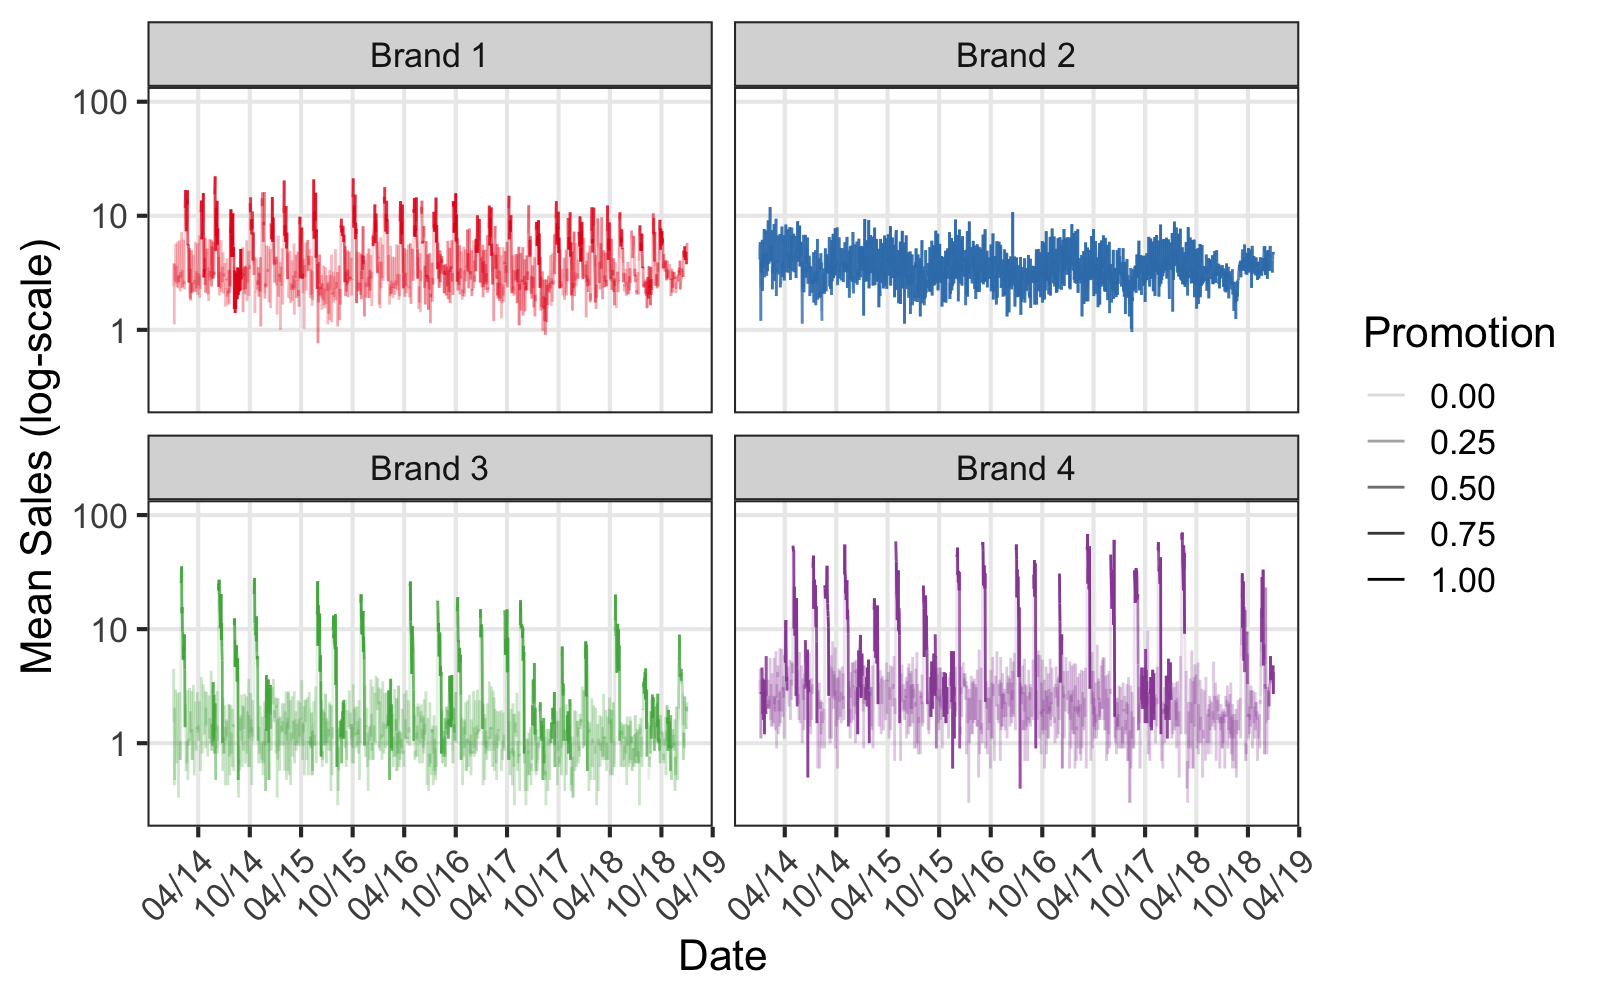
\includegraphics[width=0.6\linewidth]{figures/logscale_facet_meanSales.png}
    \caption{Mean sales by brand on a log-scale with promotion as a proportion of brand-level items on promotion.}
    \label{fig:logscaleMeanSales}
\end{figure}

\noindent We can also visualize correlation of items within each brand with Figure~\ref{fig:heatmap}. Strong positive correlations suggest that promotional or temporal effects may extend across multiple items within a brand.

\begin{figure}[ht]
    \centering
    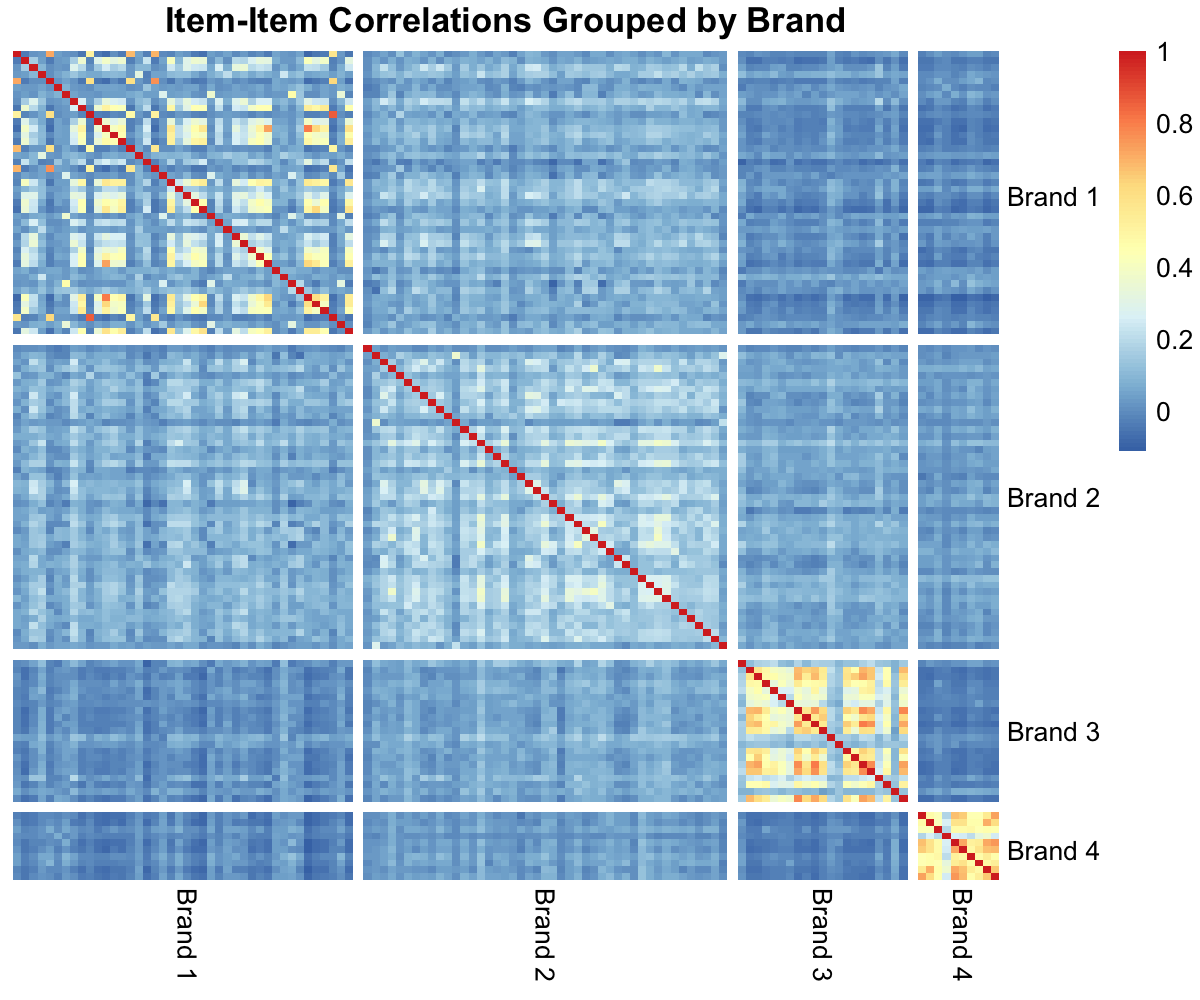
\includegraphics[width=0.5\linewidth]{figures/heatmap.png}
    \caption{Heatmap displaying within-brand item-level correlations}
    \label{fig:heatmap}
\end{figure}

\subsection*{Research Questions}

\noindent The goal of this report is to investigate the following:

\begin{enumerate}
    \item How do temporal trends and promotion-sales relationships vary across the four pasta brands?
    \item Can we improve forecasting of sales by accounting for the hierarchical structure in the data compared to simply modeling each brand (and item) independently?
\end{enumerate}

\noindent We compare likelihood-based models (BFGS), Bayesian inference (MCMC, Metropolis-Hastings), and machine learning benchmarks (Random Forests), using out-of-sample mean squared error (MSE) as the main evaluation metric.

\section{Methods}

\subsection{Motivation}
To address our research goals, we consider several variations of time series models. The key commonality behind these model is that they all use information from the previous history of sales as a predictor of the current sales for a given item. These types of models are known as autoregressive (AR) models, which have been widely-used across disciplines for time series forecasting \citep{hamilton2020time}. Additionally, our models all include the current promotion status for a given item as a predictive of the current sales for that item. \\

\noindent One issue that arises from this dataset is that the sales outcomes are discrete counts. Classical AR-based approaches, such as the Autoregressive Moving Average (ARMA), make normality assumptions about the current count outcomes given past history, but the model support is over the real line with a constant variance assumption. However, given the discrete, non-negative integer data, a more appropriate assumption in our case is that the sales are distributed according to a Poisson distribution. We can then incorporate the autoregressive structure into the Poisson mean parameter, leading to a Poisson autoregressive model (PAR), formulated below. To deal with the inherent correlations across items within each brand, we also formulate a variation of this PAR model that can jointly model sales across all items, after accounting for similarities by brand.


\subsection{Autoregressive moving-average model (ARMA) for single item modeling}
\noindent We first consider the classic ARMA model for time series data. Formally, an ARMA(p,q) model is given by
\begin{align*}
    & y_t = \alpha + \sum_{l=1}^p\beta_l y_{t-l} + \gamma x_t+ \epsilon_t +\sum_{s=1}^q \epsilon_{t-s} \theta_{s}
    \\ &\epsilon_t\overset{i.i.d.}{\sim} N(0,\sigma^2)
\end{align*}
where $y_t$ is the sales at timepoint $t$, $x_t$ is the promotion indicator at time $t$, and $\epsilon_t$ is so-called i.i.d. white-noise.

\subsection{Poisson autoregression (PAR)}

\noindent For a given item, denote the sales at timepoint $t$ by $y_{t}$, where $t=1,\ldots,T$. Also let $\mathbf{x}_t$ be a control vector including promotion indicator at time $t$ (and a $1$ element for an intercept). Based on the work by \cite{brandt2001linear}, we formulate the single-item Poisson autoregression model (PAR) as

\begin{align}
    & y_{t} \sim \text{Poisson}(m_{t}) \label{eq:PAR} \\
    & m_t = \underbrace{\sum_{l=1}^{q} \beta_l y_{t-l}}_{\text{AR part}} +
\underbrace{\left(1 - \sum_{l=1}^{q} \beta_l \right)}_{\text{mixing weight}} \cdot
\underbrace{\exp( \mathbf{x}_t'\boldsymbol{\gamma})}_{\text{covariate part}} \notag
\end{align}

\noindent where $m_t$ is the mean Poisson parameter at time $t$, $\beta_l$ is the autoregressive coefficient for lag $l$ ($l=1,\ldots,q$), and $\boldsymbol{\gamma}$ represents the effect of current covariates (including promotion) on sales. The time-varying Poisson mean can be interpreted as a weighted combination of previous observations of sales and the covariates, where the exponential term comes from the $\log$ link used for Poisson regression. We impose the constraints $\beta_l \geq 0$ and $\sum_{l=1}^q \beta_l < 1$ to ensure that the AR process is stationary (i.e. not diverging over time).

\subsubsection{Likelihood and Gradient}

\noindent Let $\boldsymbol{\theta}$ denote the full set of model parameters. The full likelihood across all items and times is given by
\begin{align*}
    & \mathcal{L}(\boldsymbol{\theta}) =
\prod_{t=q+1}^T
\frac{m_{t}^{y_{t}} e^{-m_{t}}}{y_{t}!}
\end{align*}

\noindent The corresponding log-likelihood, used for optimization and posterior inference is
\begin{align*}
    & \log \mathcal{L}(\boldsymbol{\theta}) =
\sum_{t=q+1}^T \left[
y_{t} \log(m_{t}) - m_{t} - \log(y_{t}!)
\right]
\end{align*}
\noindent where $m_t$ is defined above. For the gradient (i.e. score function), we define $a_t = \sum_{l=1}^q \beta_ty_{t-l}$, $c_t = \exp(x_t^T\boldsymbol{\gamma})$,  $w = 1 - \sum\beta_t$, and $m_t = a_t + w \cdot c_t$. Then, the derivative of the log-likelihood with respect to $\gamma_j$ is

\begin{align*}
    & \frac{\partial{\log\mathcal{L}}}{\partial\gamma_j} = \sum_{t = q + 1}^T \left[ \frac{y_t}{m_t} - 1\right] \cdot w \cdot c_t \cdot x_{tj}
\end{align*}

\noindent and the derivative of the log-likelihood with respect to $\beta_k$ is
\begin{align*}
    & \frac{\partial{\log\mathcal{L}}}{\partial\beta_k} = \sum_{t = q + 1}^T \left[ \frac{y_t}{m_t} - 1\right] \left[ y_{t-k} - c_t\right]
\end{align*}


\subsection{Hierarchical PAR for multi-item modeling}

\noindent We consider extending Model \ref{eq:PAR} to jointly model more than one item at a time. Suppose we have $n$ items, $T$ timepoints and $B$ brands. Let $g_i \in \{1,\ldots,B\}$ denote the brand (group) to which item $i$ belongs. \\

\noindent We propose a hierarchical Bayesian extension of the PAR model, which we refer to as the Poisson Vector Autoregression (PVAR) model. The sales $y_{it}$ for item $i$ and timepoint $t$ are modeled similarly to the PAR case as

\begin{align}
    & y_{it} | m_{it} \sim \text{Poisson}(m_{it}) \label{eq:PVAR} \\
    & m_{it} = \sum_{l=1}^q \beta_{i,l} y_{i,t-l}+\left(1-\sum_{l=1}^q \beta_{i,l} \right) \exp(\mathbf{x}_{it}' \boldsymbol{\gamma}_i) \notag
\end{align}

\noindent where each item is assumed to have its own autoregressive coefficients $\beta_{i,l}$ and covariate effects $\boldsymbol{\gamma}_i$. We use the following hierarchical priors on model parameters

\begin{align*}
    & \boldsymbol{\gamma}_i \sim N(\boldsymbol{\mu}_{g_i}, \Sigma_{g_i}) \\
    & \boldsymbol{\mu}_{g_i} \sim N(\boldsymbol{\mu}_0, \Sigma_0), \ \Sigma_{g_i} \sim \text{Inv-Wishart}(\nu, \Psi) \\
    & \tilde{\boldsymbol{\beta}}_i | \tau_{g_i} \sim \text{Dirichlet}(\boldsymbol{\alpha}_{g_i}), \ \beta_{i,l}=\tau_{g_i} \tilde{\beta}_{i,l} \\
    & \boldsymbol{\alpha}_{g_i} \sim \text{Dirichlet}(\alpha_0,\ldots,\alpha_0), \ \tau_{g_i} \sim \text{Beta}(a_{\tau}, b_{\tau})
\end{align*}

\noindent where $\boldsymbol{\mu}_0$, $\Sigma_0$, $\nu$, $\Psi$, $\alpha_0$, $a_{\tau}$, and $b_{\tau}$ are fixed hyperparameters. For our analysis, we choose $\boldsymbol{\mu}_0=\boldsymbol{0}$, $\Sigma_0=\Psi=\mathbf{I}$, $\nu=2$ (1 covariate + intercept), $\alpha_0=1/q$ ($q$ is fixed lag), and $a_{\tau}=b_{\tau}=2$. Our structure of priors assume that the parameters for items within a given brand come from some common distribution. Effectively, this will pool information from within each brand when estimating the effects of previous sales and promotion for each item. We use Dirichlet and Beta distributions for the AR coefficients as a way to impose the constraint that $\sum_{l=1}^q \beta_{i,l} < 1$, which leads to stationarity in the Poisson AR processes for each item.


\subsection{Broyden–Fletcher–Goldfarb–Shanno (BFGS)}

\noindent To estimate model parameters, we minimized the negative log-likelihood function using the Broyden-Fletcher-Goldfarb-Shanno (BFGS) algorithm. BFGS is a quasi-Newton method that iteratively approximates the inverse Hessian matrix of the negative log-likelihood function. Optimization was initialized with $\theta$ zero values, and the inverse Hessian was set to the identity matrix. At each iteration, the step direction was determined by the approximate Hessian inverse, and a line search was performed to satisfy the Armijo condition for sufficient decrease. The algorithm was terminated once the difference in the magnitude of log-likelihood between iterations was below some tolerance value, typically $10^{-5}$ or when a maximum number of iterations was reached.


\subsection{Expectation Maximization (EM)}

\noindent Not every promotion time point yields an increase in sales. For this reason, we explore using Expectation Maximization (EM) to down-weight or silence promotion time points that would otherwise be regarded as failed promotions. Here we assume that the promotion covariates $\gamma$ are confounded with some unknown effectiveness latent variable $z_i \sim \text{Bernoulli}(\pi_i)$, where $\pi_i$ represents the probability that a certain pair of items from a certain brand has a successful promotion. The EM algorithm iteratively maximizes the expected complete-data log-likelihood, defined as

\begin{align*}
    Q(\theta | \theta^{(k)}) = E_{z_k | \boldsymbol y, \theta^{(k)}} [\log \mathcal{L}(\boldsymbol y, z_{k = \hat k} | \boldsymbol{\theta})]
\end{align*}

\noindent For the E-step, we computed the conditional expectation of the complete-data log-likelihood given the observed data and current parameters. Within the M-step, we maximized the Q-function with respect to $\theta$ using the BFGS algorithm. Iterations of the EM algorithm were run until the relative change in log-likelihood was below some tolerance value.

\subsection{Markov Chain Monte Carlo (MCMC)}

\noindent We implemented a Metropolis-within-Gibbs MCMC algorithm to sample from the posterior distributions of model parameters for Model \ref{eq:PAR} and Model \ref{eq:PVAR}. The full conditional distributions for the autoregressive coefficients ($\beta$) and covariate effects ($\gamma$) did not have closed forms, necessitating the use of Metropolis-Hastings (MH) sampling within the Gibbs algorithm. Furthermore, the parameters associated with the AR coefficients were subject to simplex constraints. To apply the MH step for these terms, we transformed to the unconstrained space using a log-ratio transformation, generated a proposed value from a proposal distribution, then transformed the proposed value back into the constrained space. The corresponding acceptance ratio for the MH step accounted for the Jacobian associated with the inverse transformation. For all Metropolis-Hastings steps, we use a Normal proposal density with variance $0.05$ and mean set to the current value of the (transformed) parameter. Gibbs steps were used for the $\boldsymbol{\mu}_{g_i}$ and $\Sigma_{g_i}$, which represent the mean and variance of covariate effects for items within brand $g_i$ and have standard closed-form conditional posteriors.

\subsection{Model Evaluation}

\noindent To diagnose the performance of the MCMC sampling, we visually assessed traceplots for key model parameters, including the AR terms and the effect of promotion. We further stratified by brand to assess potential brand-specific issues with MCMC mixing. These traceplots are shown in Supplementary Materials. \\

\noindent For all forecasting schemes, we applied a 80\%-20\% training-test split, where the first 80\% of timepoints for each item were used for model training. We then performed two types of forecasting on the test set using trained model estimates. The first type was {\it 1-step forecasting}, where we compute the predicted value of $y_{t+1}$ given the previous $q$ time points of the observed sales data. In this sense, the 1-step forecasting still relies on training data to estimate model parameters, but makes use of the test set outcomes when generating predictions. The second type of forecasting we used was {\it $H$-step forecasting}, where $H$ was set to the size of the test set. This involves predicting the entire span of time points in the test set, only using the training set information. To perform this step using the PAR model, for instance, we replace the autoregressive term $\sum_{l=1}^q \beta_l y_{t-l}$ with $\sum_{l=1}^q \beta_l \hat{m}_{t-l}$, where $\hat{m}_{t}$ is the estimate for the Poisson mean obtained only from the training data. After generating 1-step and H-step forecasts, we calculate the Mean Squared Error (MSE) and Poisson Deviance to compare model performance. This process was repeated across all items in the dataset.

\subsection{Random Forest}
\noindent We incorporate Random Forest to implement one-step and H-step prediction on the item level. The following elaboration is based on the data of first item of the Brand 1. \\

\noindent We first fit the one-step model. Since we are interested in the effect of promotion and brand on items' sales over time, except for the existing promotion information, we also created \textit{lag1}(yesterday's sale), \textit{lag7}(sales from a week ago), \textit{TotalB1} (Total sales of all items within the same brand at that day), and \textit{Roll7totalB1}(Mean sales of all items within same brand in the last a week) as the model features. In addition, we added some other features that might be informative, such as \textit{Month} (In which month)and \textit{dow} (which day of the week). \\

\noindent After the feature specification, We split the first 80 \% as training data and remaining 20\% as test data. The next step for one-step model is hyperparameter tuning. We search the grid based on out-of-bag RMSE metric to find the best combination of \texttt{mtry}(The number of randomly selected features considered for splitting at each node) and \texttt{mini.node.size} (minimum number of observations for a tree to consider splitting.), and set the \texttt{num.tree} and \texttt{sample.fraction} to default values. The Final set-up is \texttt{mtry =4},  \texttt{mini.node.size =10}, \texttt{num.tree = 500} and \texttt{sample.fraction = 1}. We were then able to fit the one-step model, and do the prediction on the test set. \\

\noindent Based on the one-step prediction model, we can set up the H-step prediction. So instead of directly predicting the next timepoint based on current information, H-step prediction sequential prediction where the estimated $\hat{y}_t$ replaces the actual $y_t$ for future steps. The features remain the same as in the one-step model. Take \textit{lag1} as an example showing how we did this. Denote $y_T$ as the sales on the last time point, $T$, of the training set, then we feed $y_T$ back to the one-step model to predict $\hat{y}_{T+1}$, to predict $\hat{y}_{T+2}$, we now can only use $\hat{y}_{T+1}$ to feed the one step model. \\

\noindent Here predictions are generated from time $t+1$ to $t+H$, where $H$ equals the number of observations in the test set.


\section{Results}

\subsection{Estimation}

\subsubsection{ARMA}
\noindent We fit each brand item pair with ARMA model. We show here the results of item $1$ in brand $1$ for example. \\

\noindent It is often critical to figure out the order of the ARMA model. We hence first use partial autocorrelation function (PACF) to determine the order in AR and use autocorrelation function (ACF) to determine the order in MA. Figure~\ref{fig:acf} is one example of sample PACF and ACF. We can see that the PACF on the left panel shows significant spikes at lags $1$, $2$, and $4$, then cuts off, pointing us toward an AR(4) structure. Meanwhile, the left panel of ACF plot exhibits a slow exponential decay out to lag $8$ or so,  indicating a moving-average component of order at least about $4$ or $5$. Putting these clues together, we tentatively select an ARMA(4,5) specification. \\

\begin{figure}[!ht]
\centering
\begin{tikzpicture}
        \node[below right,inner sep=0] (image_11) at (0,0) 
        {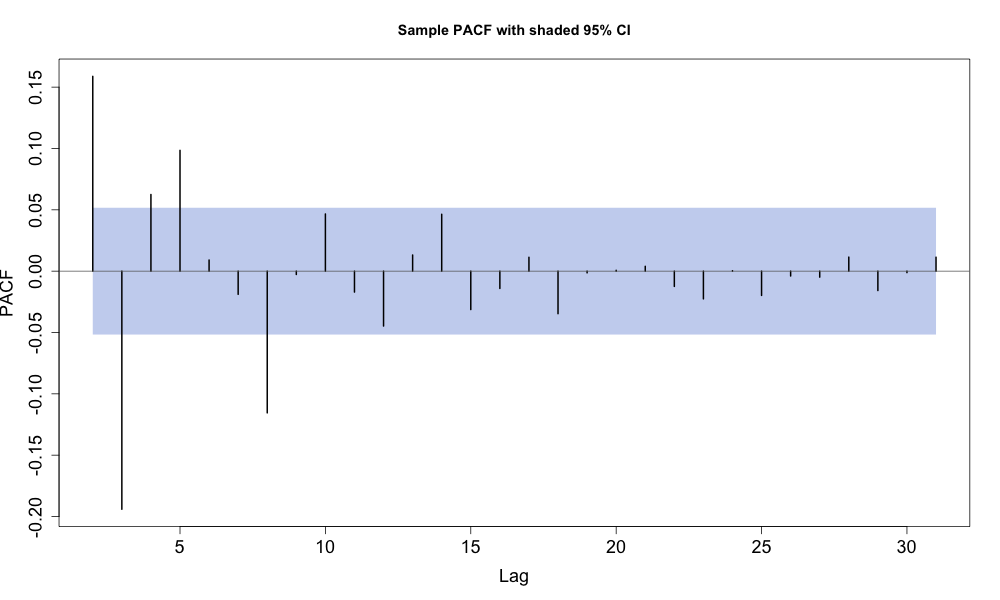
\includegraphics[width=0.4\textwidth, trim=0 0 0 0, clip]
            {figures/PACF.png}
        };         \begin{scope}[
        shift={($(image_11.south west)$)},
        x={($0.1*(image_11.south east)$)},
        y={($0.1*(image_11.north west)$)}]
              \node[above] at ($(5.3,-1)$){\textbf{PACF}};
    \end{scope} 

            \node[below right = 0 and 0.5 of image_11.north east,inner sep=0] (image_12) at (image_11.north east) 
        {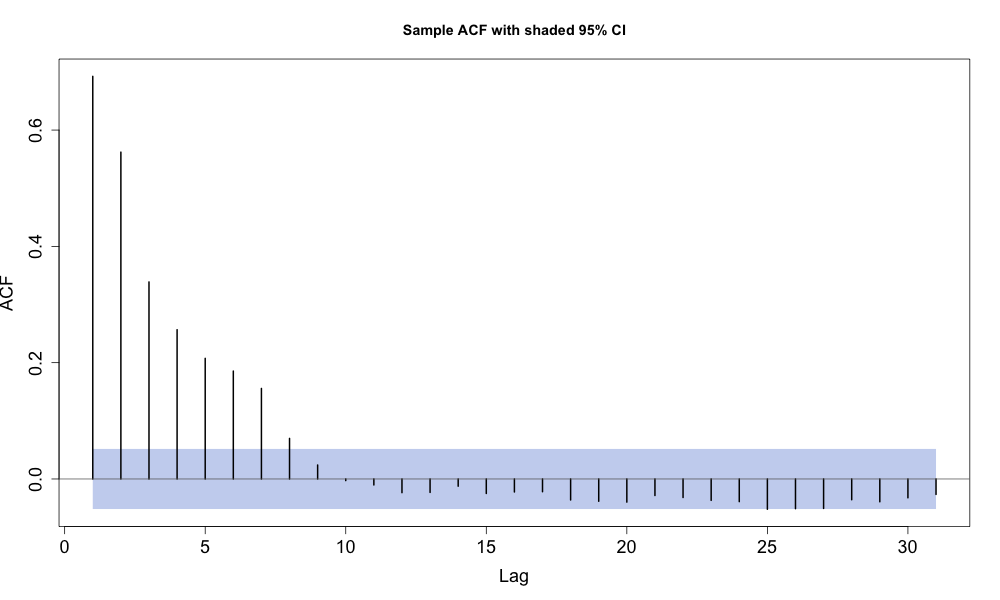
\includegraphics[width=0.4\textwidth, trim=0 0 0 0, clip]
            {figures/ACF.png}
        };        
        \begin{scope}[
        shift={($(image_12.south west)$)},
        x={($0.1*(image_12.south east)$)},
        y={($0.1*(image_12.north west)$)}]
              \node[above] at ($(5.3,-1)$){\textbf{ACF}};
    \end{scope}
\end{tikzpicture}
\caption{Sample PACF and ACF for item 1 in brand 1. The shaded blue areas are the $95\%$ confidence band.}
\label{fig:acf}
\end{figure}

\noindent After fitting the ARMA(4,5) model, we check the residuals. We first check the autocorrelations again. Figure~\ref{fig:racf} shows the residual ACF with $95\%$ confidence bands. Virtually, all autocorrelations lie within the bounds, indicating no remaining serial dependence. Moreover, the Ljung–Box test on the residuals yields a p-value of 0.519, so we cannot reject the null of no autocorrelation. We also run a Shapiro–Wilk test, however, the p-value ($2e-16$) is extremely small  as expected, our response is count data. This highlights a limitation of the basic ARMA approach, but as a first approximation it still captures much of the serial pattern in pasta sales.

\begin{figure}[!ht]
\centering
\begin{tikzpicture}
        \node[below right,inner sep=0] (image_11) at (0,0) 
        {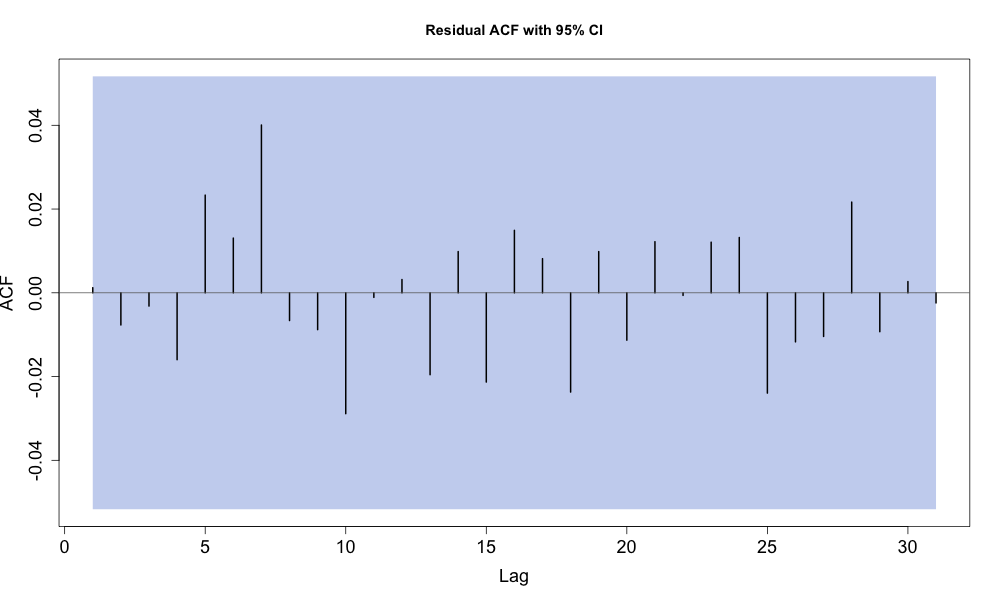
\includegraphics[width=0.6\textwidth, trim=0 0 0 0, clip]
            {figures/res_ACF.png}
        };         \begin{scope}[
        shift={($(image_11.south west)$)},
        x={($0.1*(image_11.south east)$)},
        y={($0.1*(image_11.north west)$)}]
              \node[above] at ($(5.3,-1)$){\textbf{Residuals ACF}};
    \end{scope}         
\end{tikzpicture}
\caption{Residuals ACF for item $1$ in brand $1$ after fitting ARMA(4,5). The shaded blue areas are the $95\%$ confidence band.}
\label{fig:racf}
\end{figure}

\noindent Furthermore, estimates for all the parameters except for $\sigma^2$ in the ARMA model are shown in figure~\ref{fig:coefarma} for item $1$ in brand $1$. We can see most of the coefficients are statistically significant, confirming our model structure. Especially, we see that $\gamma$ is statistically significant and is also greater than $0$, indicating a true positive correlation between promotion and sales of pasta.

\begin{figure}[!ht]
\centering
\begin{tikzpicture}
        \node[below right,inner sep=0] (image_11) at (0,0) 
        {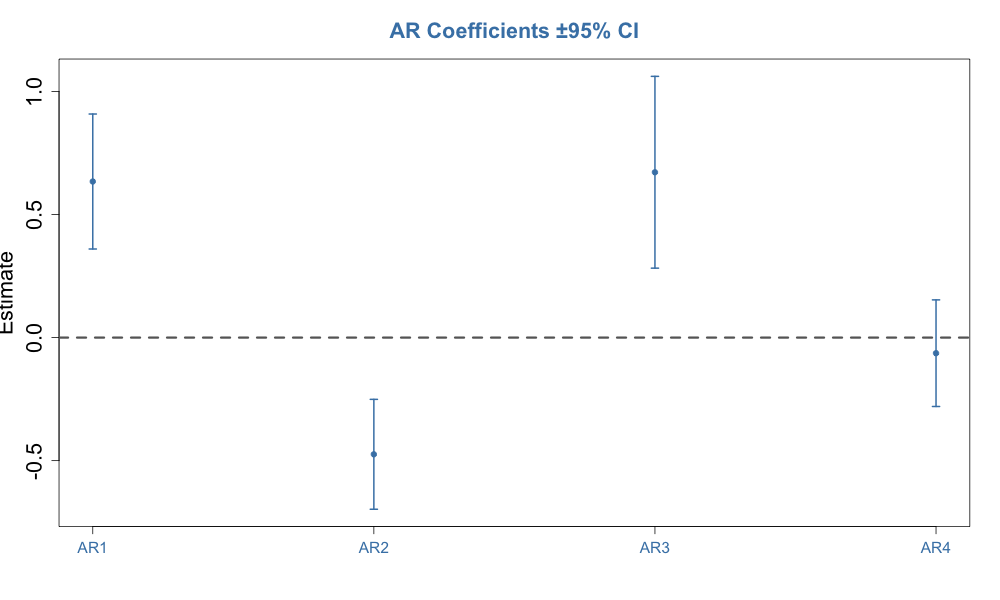
\includegraphics[width=0.3\textwidth, trim=0 0 0 0, clip]
            {figures/coef_AR.png}
        };         \begin{scope}[
        shift={($(image_11.south west)$)},
        x={($0.1*(image_11.south east)$)},
        y={($0.1*(image_11.north west)$)}]
              \node[above] at ($(5.3,-1)$){\textbf{AR}};
    \end{scope} 

            \node[below right = 0 and 0.5 of image_11.north east,inner sep=0] (image_12) at (image_11.north east) 
        {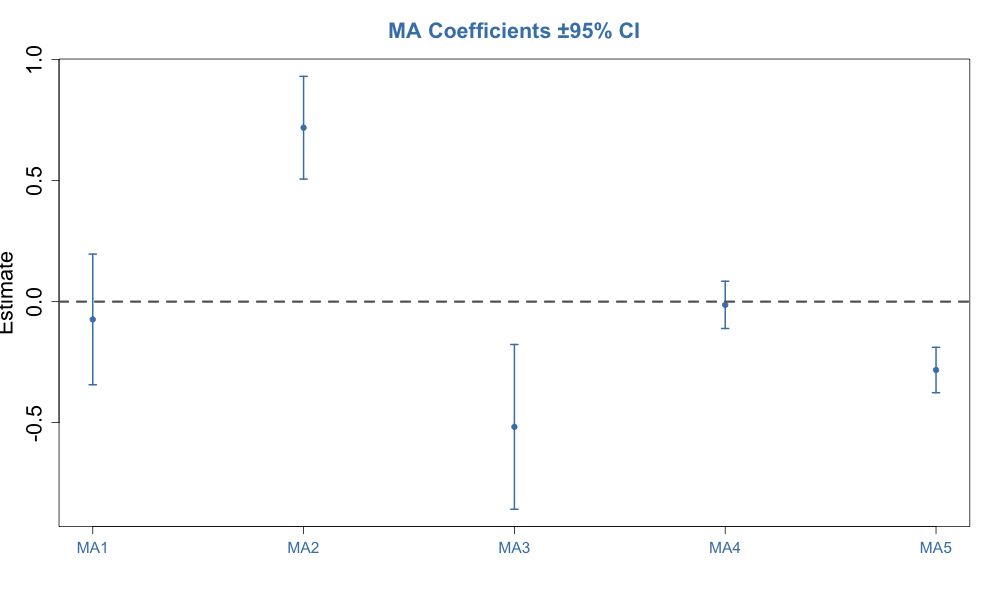
\includegraphics[width=0.3\textwidth, trim=0 0 0 0, clip]
            {figures/coef_MA.png}
        };        
        \begin{scope}[
        shift={($(image_12.south west)$)},
        x={($0.1*(image_12.south east)$)},
        y={($0.1*(image_12.north west)$)}]
              \node[above] at ($(5.3,-1)$){\textbf{MA}};
    \end{scope}


                \node[below right = 0 and 0.5 of image_12.north east,inner sep=0] (image_13) at (image_12.north east) 
        {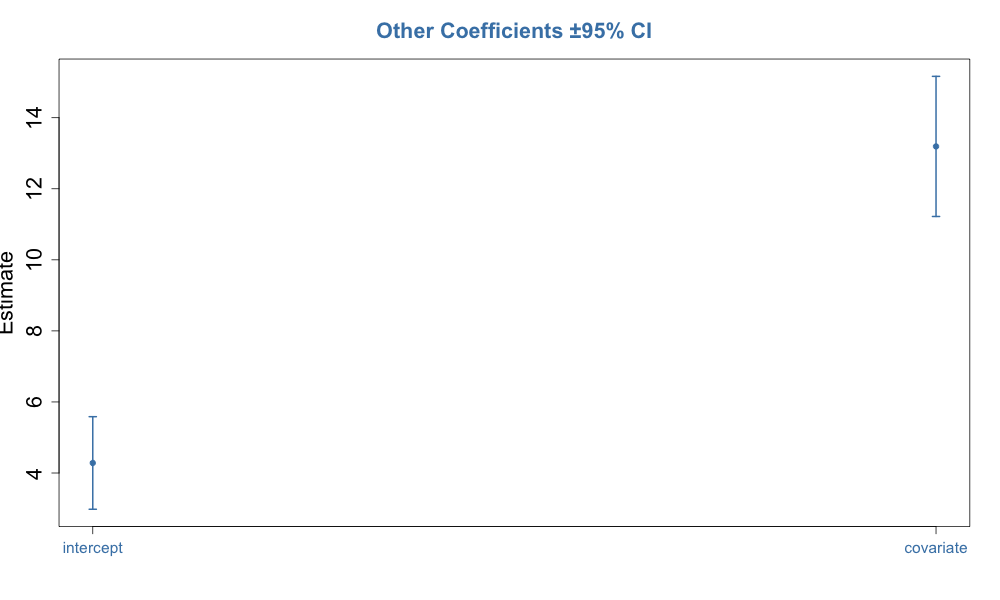
\includegraphics[width=0.3\textwidth, trim=0 0 0 0, clip]
            {figures/coef_other.png}
        };        
        \begin{scope}[
        shift={($(image_13.south west)$)},
        x={($0.1*(image_13.south east)$)},
        y={($0.1*(image_13.north west)$)}]
              \node[above] at ($(5.3,-1)$){$\alpha$ and $\gamma$};
    \end{scope}
\end{tikzpicture}
\caption{Estimated coefficients with $95\%$ confidence band for item $1$ in brand $1$.}
\label{fig:coefarma}
\end{figure}


\subsubsection{Bayesian PAR and PVAR}
\noindent We performed MCMC sampling on all $118$ items using both the item-by-item PAR Model (Model \ref{eq:PAR}) and the multi-item PVAR Model (Model \ref{eq:PVAR}). Both sets of models included AR terms up to lag $5$, an intercept term, and a promotion effect. Estimates for model parameters were obtained by averaging the post-burn-in MCMC samples (total number of MCMC iterations = $10,000$, burn-in set to $5,000$). \\

\noindent Estimates for the item-specific AR terms ($\boldsymbol{\beta}$), stratified by brand, are shown in Figure \ref{fig:AR-Est}. The leftmost box plots for each brand correspond to $\beta_1$ and the rightmost box plot corresponds to $\beta_5$. For both models, $\beta_1$ had the largest average estimate across items, with comparably low estimates for the other $\beta_q$. This result is consistent with the ACF shown in Figure \ref{fig:acf}, and is a common finding for time series data. Additionally, we find that the PVAR model led to smaller variance across items in estimated $\beta$ values, which was due to information pooling within each brand. Notably, Brand 2 $\beta$ estimates within the PVAR model are close to zero in comparison to the PAR model, signifying a minimal dependence on previous history of sales for that brand. For the remaining brands, we find visual evidence of differences in the distribution of autoregressive term estimates (e.g. brand 4 tends to have the largest AR-1 effect), but do not rigorously test for significant differences in this analysis. \\

\noindent Estimates for the promotion effects, ($\gamma_1$) are shown in Figure \ref{fig:Promo-Est} for each item and model, again stratified by brand. Each box plot represents the estimate of promotion for a given item belonging to a certain brand. We find Brand 2 has the highest variance in parameter estimates in both the PAR and PVAR models compared to all other brands. We suspect this discrepancy is due to the average investment in an item for brand 2 is approximately 70\%, whereas the average investment for the other brands was less than 20\%. Investment here is calculated as the proportion of days a particular brand item was promoted over the course of the time series. 

\begin{figure}
    \centering
     \begin{subfigure}[b]{0.48\textwidth}
         \centering
        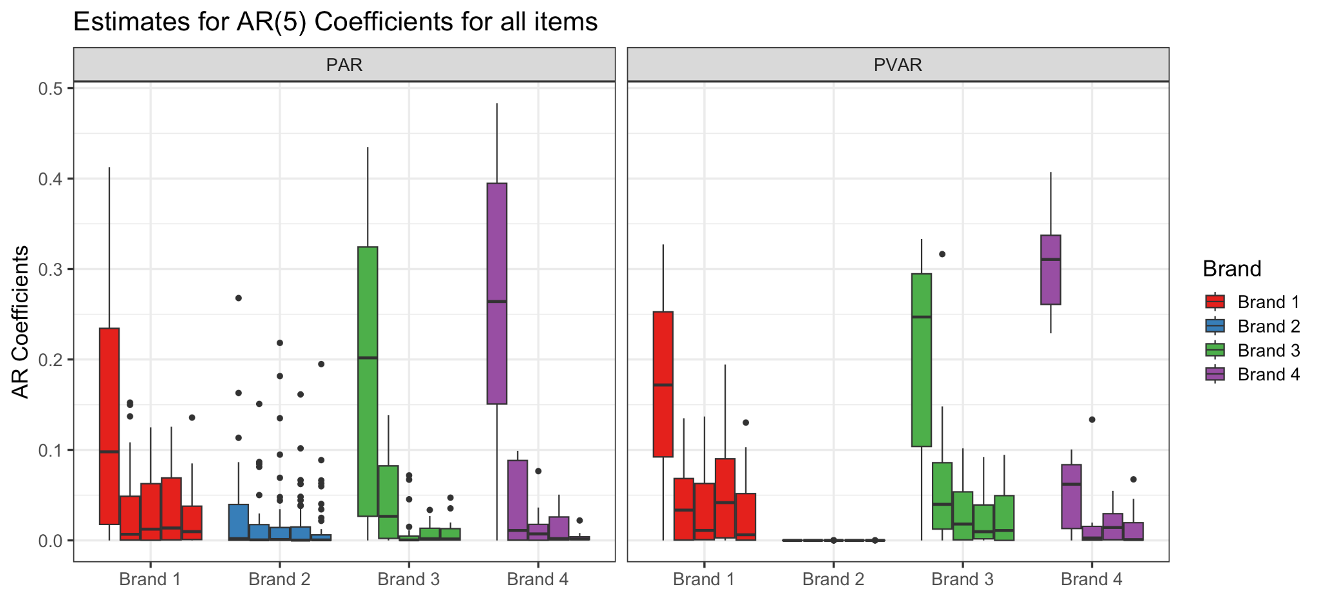
\includegraphics[width=1\linewidth]{figures/Bios735-AR-Estimates.png}
        \caption{Item-level AR term estimates for 5 lag points for the PAR and PVAR models obtained using MCMC}
        \label{fig:AR-Est}
    \end{subfigure}
    \hfill
     \begin{subfigure}[b]{0.48\textwidth}
         \centering
         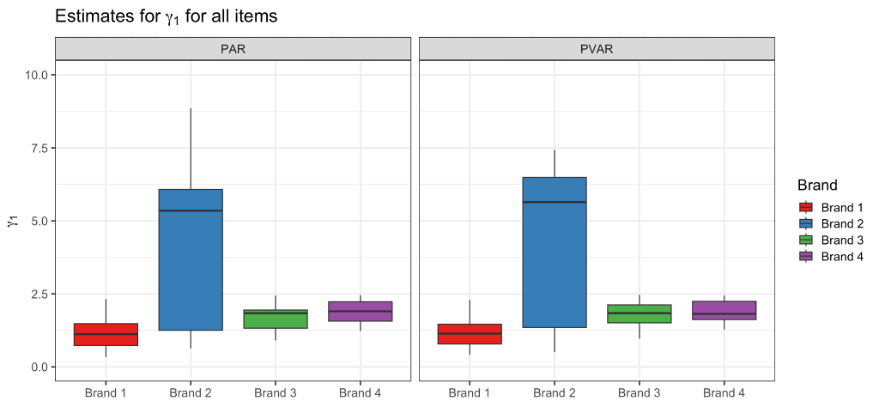
\includegraphics[width=1\textwidth]{figures/Bios735-Promotion-Effect-estimate.png}
         \caption{Item-level effects of promotion from PAR and PVAR models obtained using MCMC}
         \label{fig:Promo-Est}
     \end{subfigure}
\end{figure}

\subsubsection{EM - Estimating Effective Promotions}

\noindent Each brand item had parameters initially estimated through BFGS assuming a 5 time point lag and using an intercept and promotion as covariates to the model. The EM algorithm was run on each brand item until the relative change in log-likelihood was below $10^{-6}$. 

\begin{figure}[!ht]
    \centering
    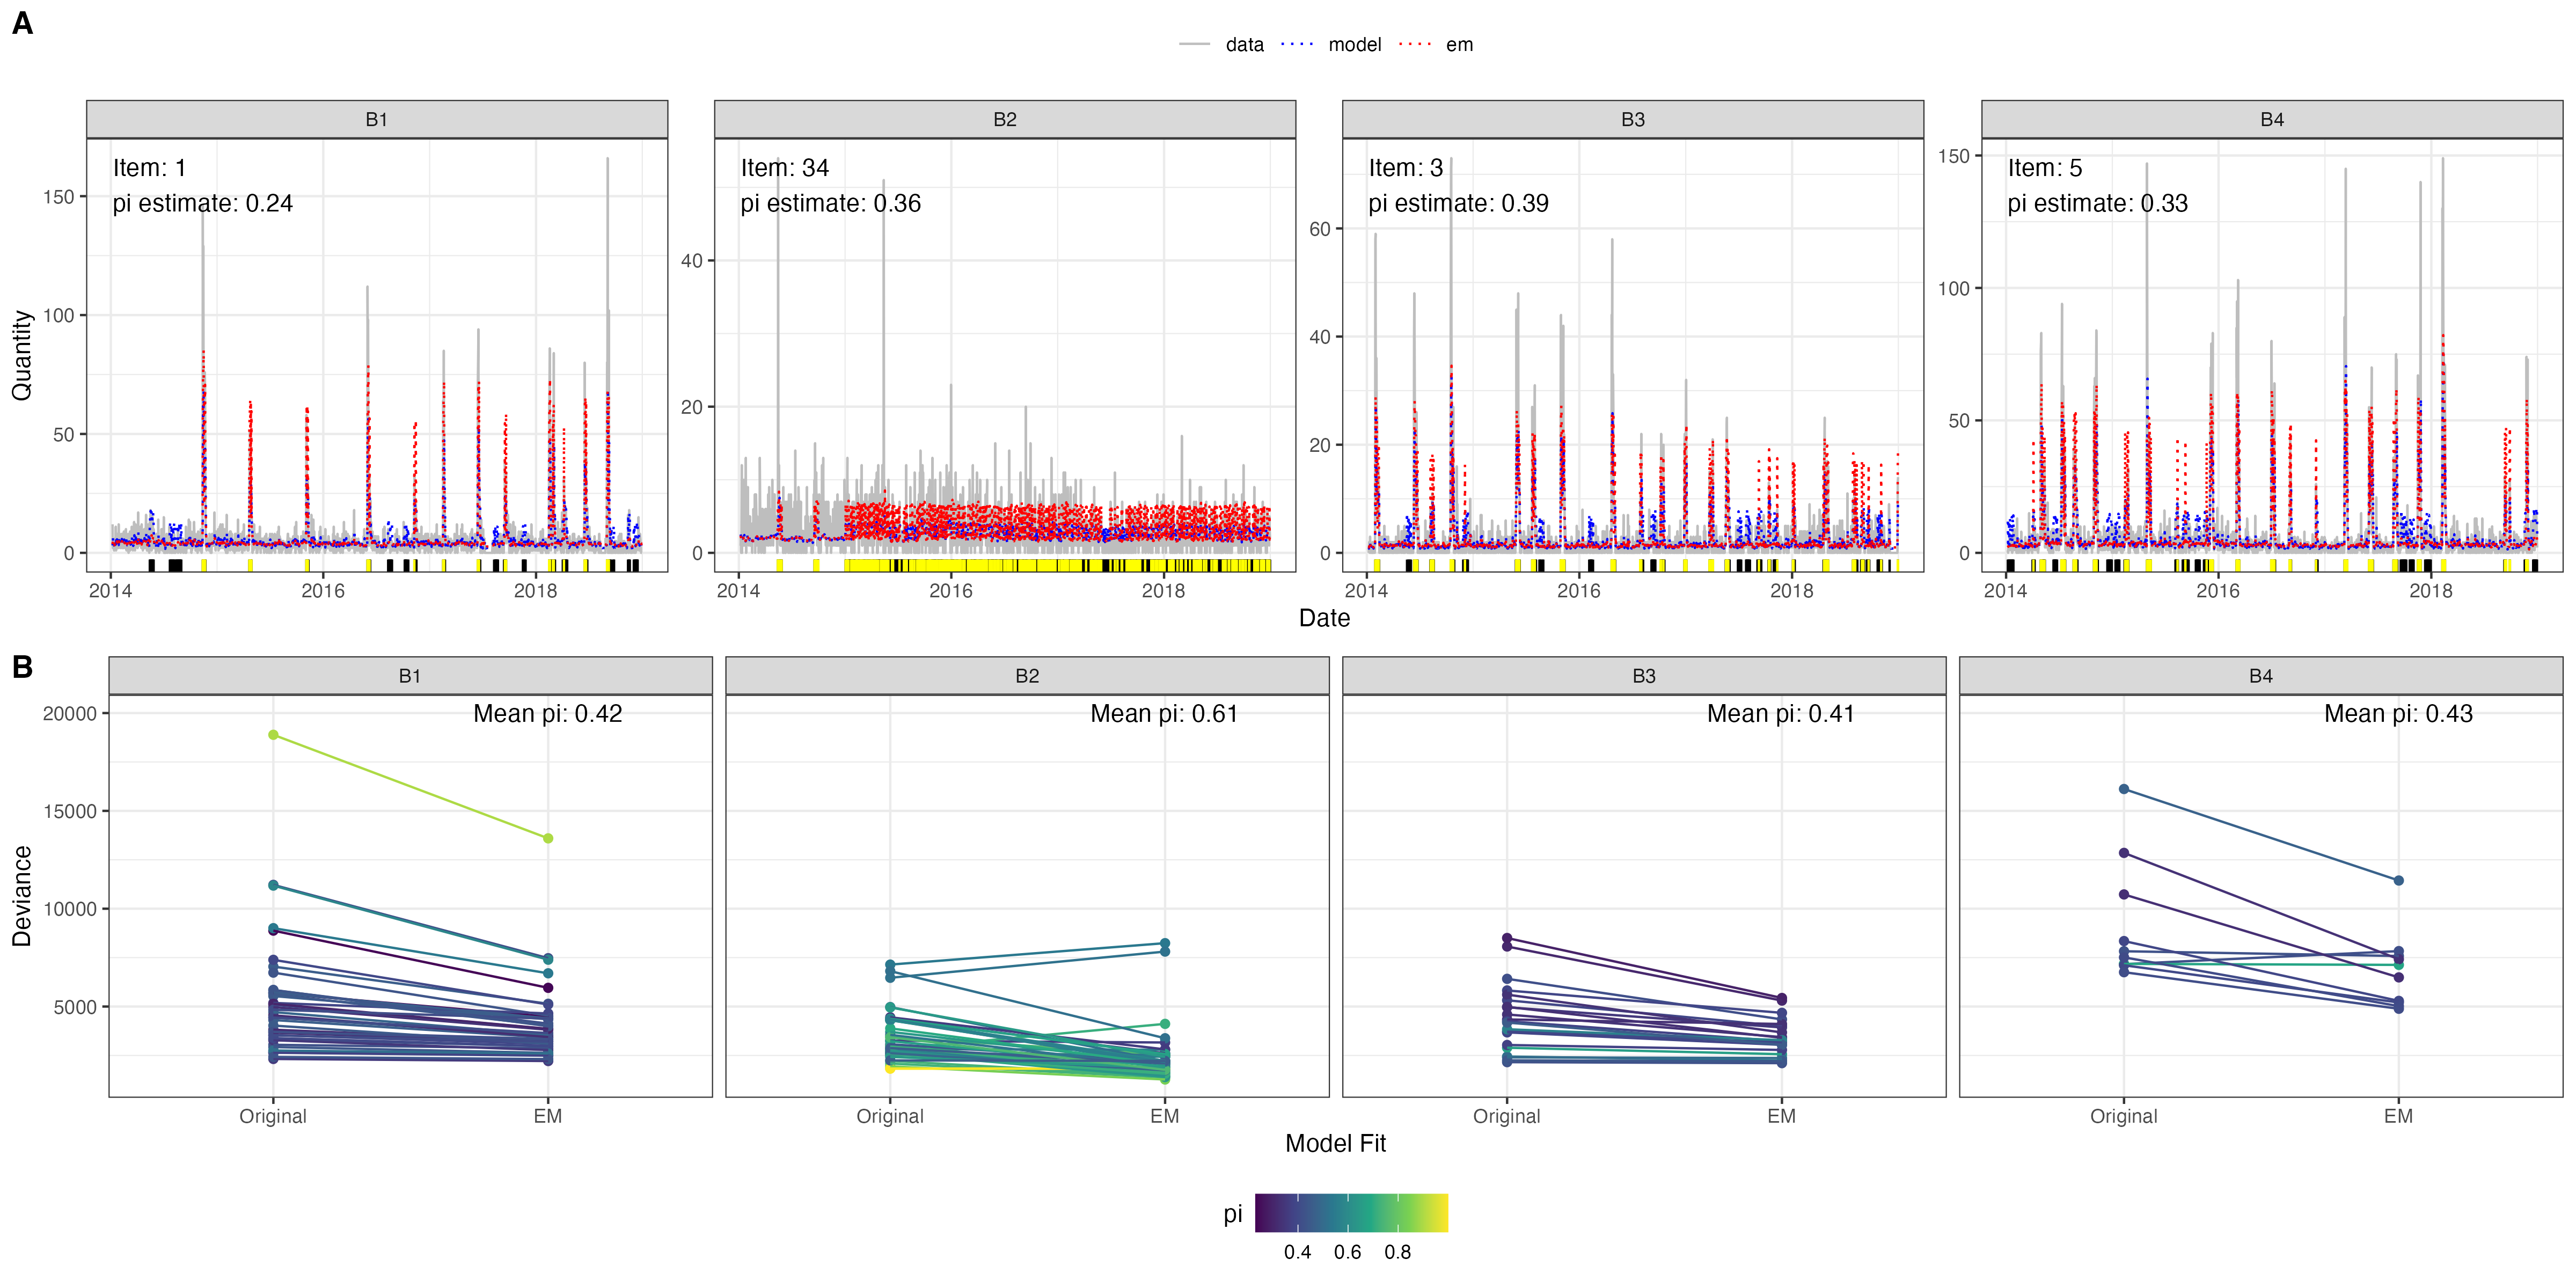
\includegraphics[width=0.9\linewidth]{figures/em_results.png}
    \caption{EM results of fitting each brand item using BFGS. Panel A: A time series of one representative example item from each brand. Grey lines indicate original observed data. Blue dotted lines indicate initial BFGS fit mean estimates. Red dotted lines indicate final mean fits after latent variable estimation. Rug marks indicate days in which a promotion occurred, while yellow marks indicate days that were effective. Panel B: deviance of the initial model estimates compared to the EM model estimates. Each brand item is colored by their estimated $\pi_i$ from EM.}
    \label{fig:EM-Est}
\end{figure}

\noindent Representative samples from each brand are shown in Figure \ref{fig:EM-Est} Panel A. The Expectation-Maximization (EM) algorithm was generally effective in improving model fit relative to the initial parameter estimates obtained via BFGS optimization. Across all brands, EM iterations consistently reduced the model deviance, indicating improved agreement between the fitted model and the observed data, with a few exceptions as seen in Figure \ref{fig:EM-Est} Panel B. \\

\noindent Analysis of the estimated latent variables $z_i$, representing the effectiveness of promotions on specific days, revealed that the inferred promotion success probabilities $\pi_i$ were typically around 0.40. That is, on average, a given brand promotion was estimated to be effective approximately 40\% of the time. An exception was observed for Brand 2, which exhibited a substantially higher promotion success rate of approximately 60\%. Notably, Brand 2 also had a much higher overall frequency of promotions, with an average promotion rate exceeding that of other brands by more than a factor of three. This disparity may challenge the ability for the EM model to estimate days effected by promotion and those due to natural sale frequency.

\subsection{Forecasting}

\subsubsection{ARMA}

\noindent To illustrate the out-of-sample performance of ARMA(4,5) model, we evaluate the forecasts on our hold-out test set. To be specific, we split the data set into training set and test set, with the first $80\%$ time points in the training set and the remaining $20\%$ time points in the test set. Figure~\ref{fig:armapred} shows the performance of prediction in detail. On the left is the one-step-ahead prediction: in most days, the forecast closely tracks the true sales spikes. On the right is the H-step forecast, we can see the performance degrades slightly as the horizon increases, but the model seems to still identify the timing of demand surges. 

\begin{figure}[!ht]
\centering
\begin{tikzpicture}
        \node[below right,inner sep=0] (image_11) at (0,0) 
        {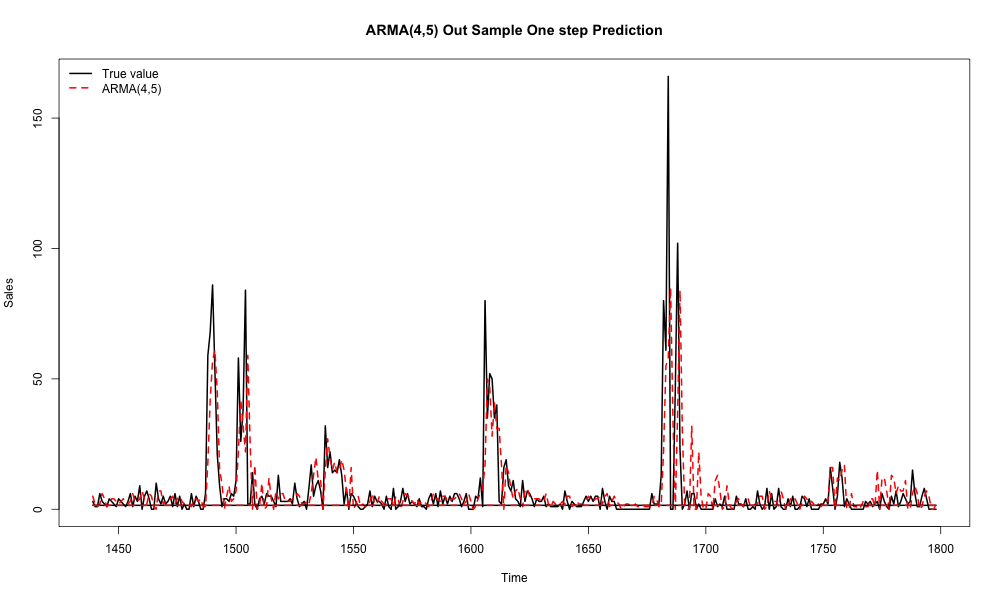
\includegraphics[width=0.45\textwidth, trim=0 0 0 0, clip]
            {figures/ARMA_pred.png}
        };         \begin{scope}[
        shift={($(image_11.south west)$)},
        x={($0.1*(image_11.south east)$)},
        y={($0.1*(image_11.north west)$)}]
              \node[above] at ($(5.3,-1)$){\textbf{One-step}};
    \end{scope} 

            \node[below right = 0 and 0.5 of image_11.north east,inner sep=0] (image_12) at (image_11.north east) 
        {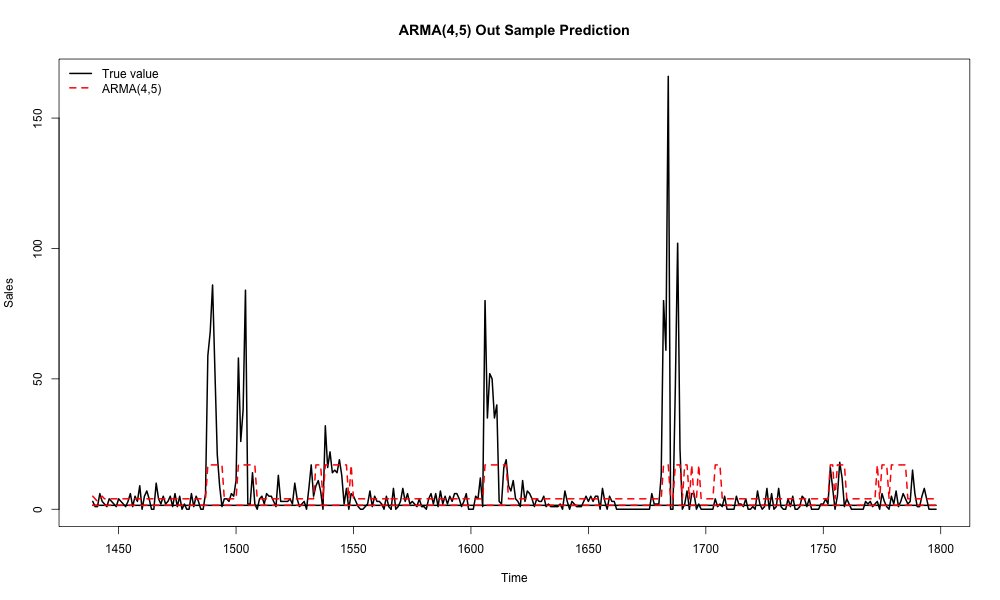
\includegraphics[width=0.45\textwidth, trim=0 0 0 0, clip]
            {figures/ARMA_predsub.png}
        };        
        \begin{scope}[
        shift={($(image_12.south west)$)},
        x={($0.1*(image_12.south east)$)},
        y={($0.1*(image_12.north west)$)}]
              \node[above] at ($(5.3,-1)$){\textbf{H-step}};
    \end{scope}
                
\end{tikzpicture}
\caption{Out-sample performance on the test set of ARMA(4,5) for item 1 in brand 1. The red dashed lines are predicted values, and the black solid lines are the true values.}
\label{fig:armapred}
\end{figure}

\noindent Generally we can see the ARMA model performs well despite of some drawbacks, it can hence be treated as the baseline model.

\subsubsection{Bayesian PAR and PVAR}

\noindent The results from forecasting using the Bayesian PAR and PVAR models (Models \ref{eq:PAR} and \ref{eq:PVAR}) are shown in Figures \ref{fig:parpred}-\ref{fig:par_forecast_eval}. Figure \ref{fig:parpred} displays the 1-step and H-step forecasts for a single item, after running MCMC for the PAR and PVAR models on the training set. We visually see similar performance to the ARMA case, with relatively good performance using 1-step forecasting and moderate performance in the H-step case. The PVAR model appears to produce slightly lower forecasts around the peaks than the PAR model in this case, though the placement of those predicted peaks appears marginally better in the PVAR case. \\

\vspace{4cm}

\begin{figure}[ht]
\centering
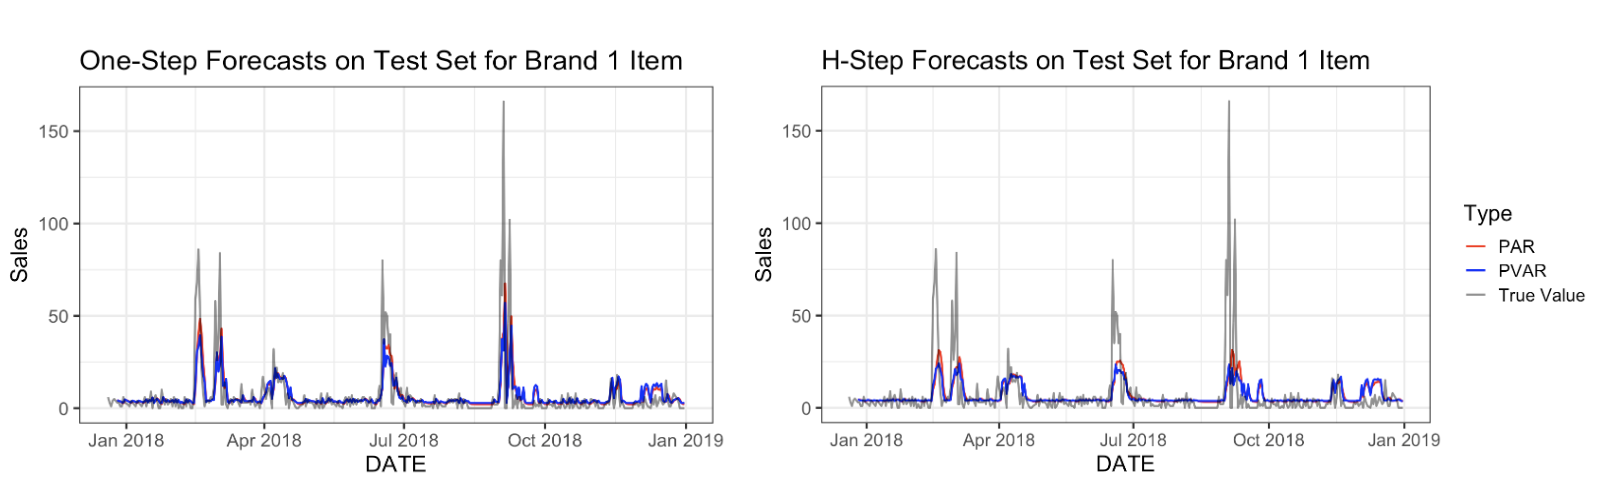
\includegraphics[width=1\linewidth]{figures/PAR_forecast.png}
\caption{Out-of-sample performance on the test set using PAR and PVAR models for item 1 in brand 1.}
\label{fig:parpred}
\end{figure}

\noindent We also display the brand-level forecasts from the PAR and PVAR model using 1-step forecasting in Figure \ref{fig:parpred_brand}. This indicate larger similar brand-level forecasting power between the PAR (non-hierarchical) and PVAR (hierarchical) models. However, we do note that the PVAR model allows for brand-level forecasting directly from model parameters, whereas the PAR model obtains these forecasts by first averaging the item-level estimates. Therefore, PVAR may be more appropriate for quantifying uncertainty about future trends at the brand-level.

\begin{figure}[ht]
\centering
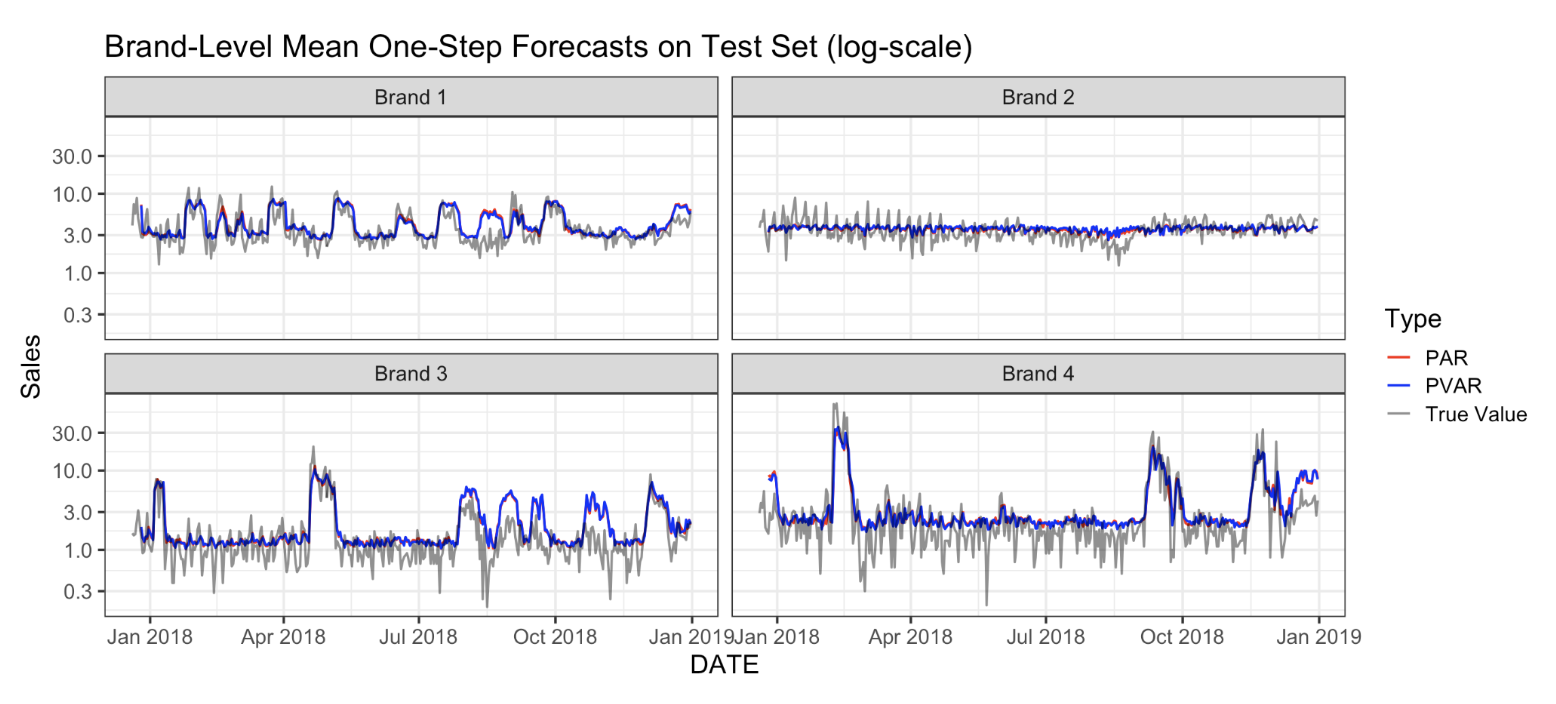
\includegraphics[width=1\textwidth]{figures/PAR_forecast_brand.png}
\caption{Out-of-sample performance on the test set using PAR and PVAR models for brand-level forecasts.}
\label{fig:parpred_brand}
\end{figure}

\noindent Lastly, we evaluated the 1-step forecasting performance for the PAR and PVAR models on all items. The resulting evaluation metrics, including Mean-Squared Error (MSE) and Poisson Deviance, are shown for all items in Figure \ref{fig:par_forecast_eval}. We find minimal differences in the forecasting performance of these two models, but do observe some additional outliers with poor predictive performance in the PAR case compared with the PVAR case. 

\vspace{2cm}

\begin{figure}[ht]
\centering
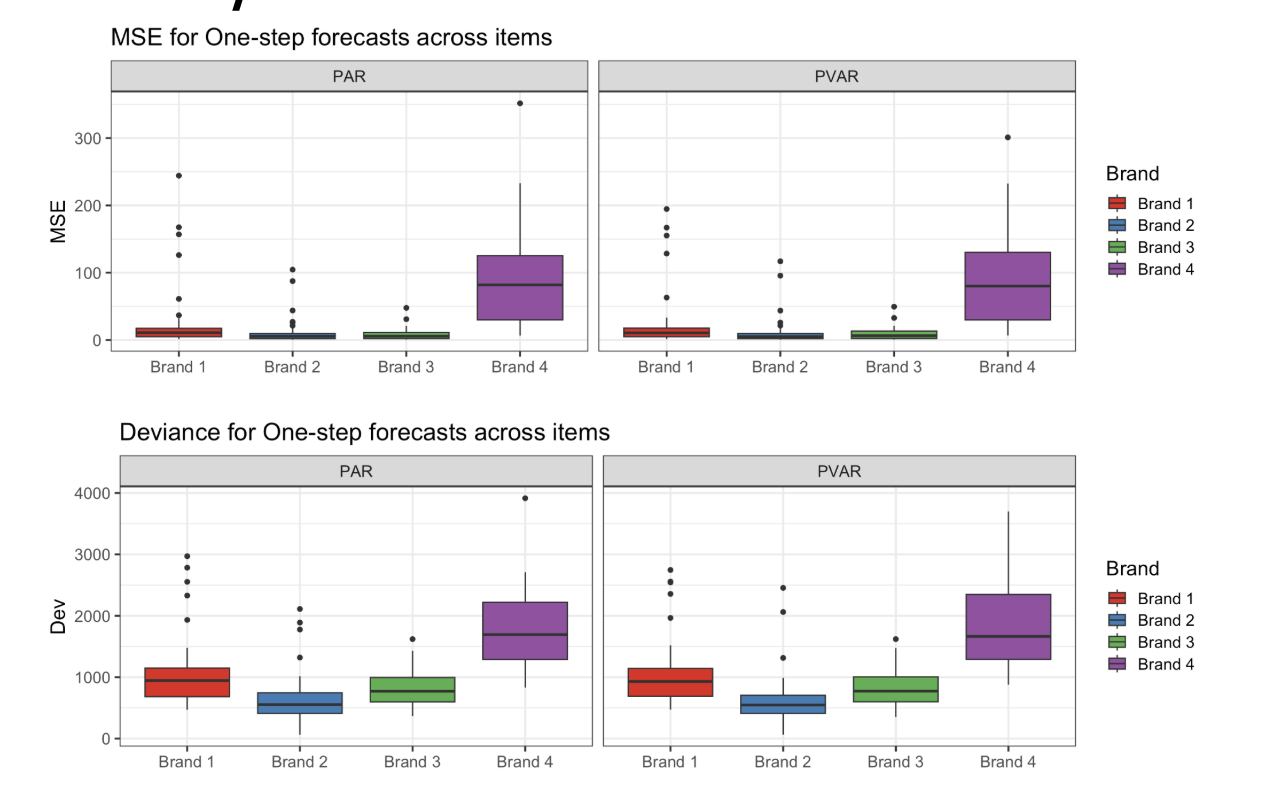
\includegraphics[width=0.8\textwidth]{figures/par_forecast_mse_dev.png}
\caption{Item-level Mean Squared Errors (MSE) and Poisson Deviance from 1-step forecasting using PAR and PVAR models}
\label{fig:par_forecast_eval}
\end{figure}


\subsubsection{Random Forest}
The prediction results based on the first item of Brand 1 using the Random Forest one-step and H-step models are shown in Figure 12. We can observe that the one-step model performs well with MSE = 109.91, while the H-step model has a poor match with the actual value, and even misses several peaks, with a corresponding MSE = 217.49. The difference in performance between these two models makes sense, since the H-step model accumulates the prediction error during the model recursion. But since we just did the prediction for one item, we also need to consider the possibility that the one-step model has an overfitting issue. \\

\noindent Besides prediction, the Random Forest algorithm also provides the Gini Importance Index for every predictor. Here, the top 3 predictors are: \textit{lag1}, \textit{TotalB1} and \textit{Promotion}. This suggests that the Random Forest-based models also identify Promotion and brand as predictors that have effect on the sales of one item. This conclusion, in some terms, coincides with the interpretation from the parametric models we fitted.

\begin{figure}[ht]
\centering
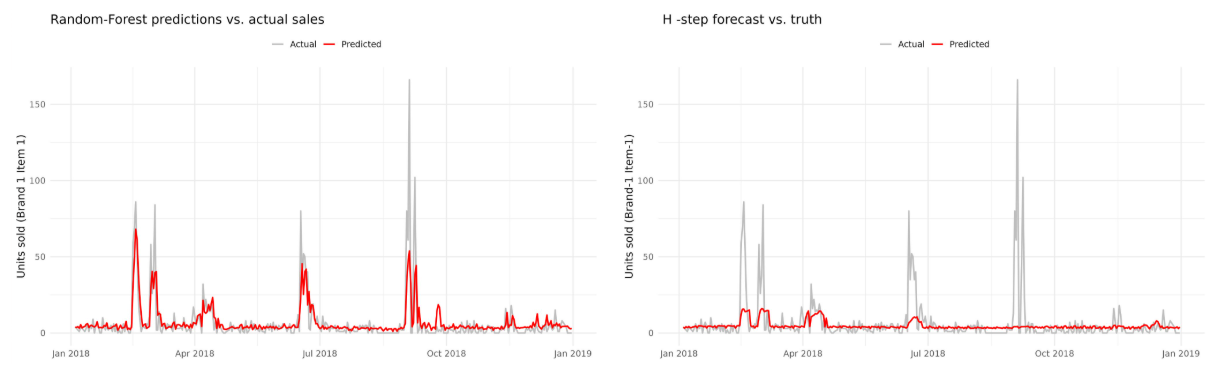
\includegraphics[width=0.9\textwidth]{figures/rf_prediction.png}
\caption{Out-of-sample performance using Random Forest for item 1 in brand 1.}
\label{fig:parpred}
\end{figure}

\section{Discussion}
\subsection{Takeaways}
\noindent Revising our research questions, we found evidence that the patterns of pasta sales over time do vary across the four brands. Furthermore, the effect of promotion on current sales varies substantially across brands, with items in brand 1 showing the weakest effect of promotion, on average. Here, we also found that brand 2 items tended to show the largest effect of promotion, but are hesitant to trust these estimates given the imbalances in the dataset. \\

\noindent For forecasting, we find similar performance for all the various models we examined, with relatively good performance using 1-step prediction and weaker performance when low to moderate performance when predicting an entire year's worth of sales. We find some marginal evidence that the hierarchical model leads to better long-term forecasting than the non-hierarchical model for certain items, though this finding was certainly not definitive. That being said, the hierarchical model offers certain unique advantages for forecasting-related tasks, such as the ability to produce brand-specific forecasts directly from model parameters. Depending on specific forecasting goals, we recommend using some version of hierarchical model for this data, since it uses more available data and can be more comprehensive to other sorts of prediction tasks such as predicting sales for an item given information about the other items.

\subsection{Limitations}

\noindent While the models developed above provide some insight into modeling and forecasting pasta sales, there are many limitations that restrict our results and insights. One limitation of our forecasting approach is that one-step forecasts rely on previous observations, which may introduce information leakage from the test set and overstate predictive performance. Our H-step forecasting does not touch the test set, but performed worse than the one-step forecasting models, and failed to adequately predict the magnitude of spikes in the data (although we did largely identify where in time these spikes occurred). Another limitation was that fitting the PAR and PVAR models was computationally intensive, even with efficiency gains from \texttt{Rcpp}-based implementations, restricting our modeling capabilities. Lastly, the data sparsity, presence of large spikes, and the imbalance of promotion events across items complicate reliable estimation and may bias effect sizes. Specifically, brand 2 promoted almost all of their items at most times, restricting our ability to estimate model parameters from brand 2. Some of these limitations can be addressed in future studies. 

\subsection{Future Directions}

\noindent One modification to our analysis that could make a significant difference in results is the distributional assumption. We have posited a Poisson distribution for our count data, where a negative binomial distribution may be more appropriate for accounting for overdispersion given the high peaks in our sales data. There are also smaller changes that could be made to improve our modeling and forecasting. This includes hyperparameter tuning for our Bayesian MCMC prior distribution. Due to time constraints, we only considered non-informative priors with a fixed set of hyperparameters. Tuning these hyperparameters, along with exploring more choices of lag,  could improve predictive performance. Relatedly, we wish to explore other options for priors which could place less restrictive assumptions on the AR terms, potentially leading to better model fitting. Additionally, we would like to finish applying the single-item Machine Learning approaches to the rest of the items in all of the brands. A comparison of these parameter estimates and forecasts will provide more insight on the existence and significance of brand-level effects in our models. 

\clearpage

\bibliographystyle{apalike}
\bibliography{ref.bib}


\newpage
\section{Supplementary Materials}

\subsection{MCMC Diagnostics}

\noindent Figures \ref{fig:traceplot_par}-\ref{fig:traceplot_pvar} show some example traceplots corresponding to the autoregressive lag-1 term and promotion effect term under the PAR and PVAR models. Each plot consists of item-level terms across 2 randomly-chosen items in each of the 4 brands.  We see that for both PAR and PVAR, the promotion effect terms appear largely convergent across items, except for the brand 2 item which shows evidence of poor mixing. This is consistent with the fact that brand 2 had highly imbalanced promotion data, which made estimation for that term difficult. Furthermore, the AR-1 terms show some evidence of poor mixing for certain items. This could be due to the high correlations between the AR-1 term and subsequent AR terms, i.e. the effect of higher lags may absorb some of the effect of lag-1 during sampling.

\begin{figure}[!ht]
    \centering
    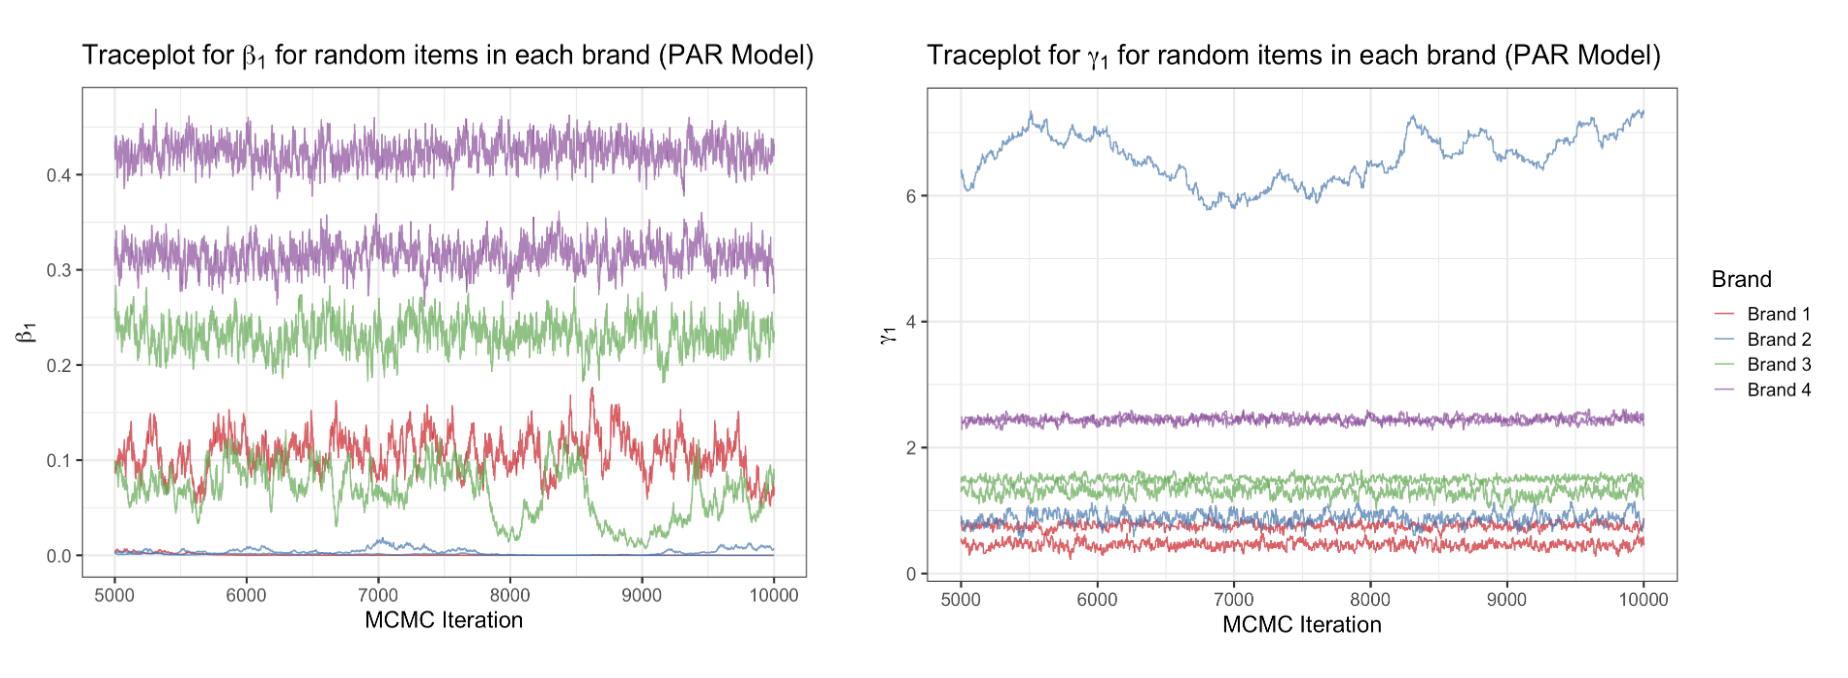
\includegraphics[width=1\linewidth]{figures/traceplot_par.png}
    \caption{Traceplots for item-level AR-1 terms and promotion effect terms using the single-item PAR model.}
    \label{fig:traceplot_par}
\end{figure}

\begin{figure}[!ht]
    \centering
    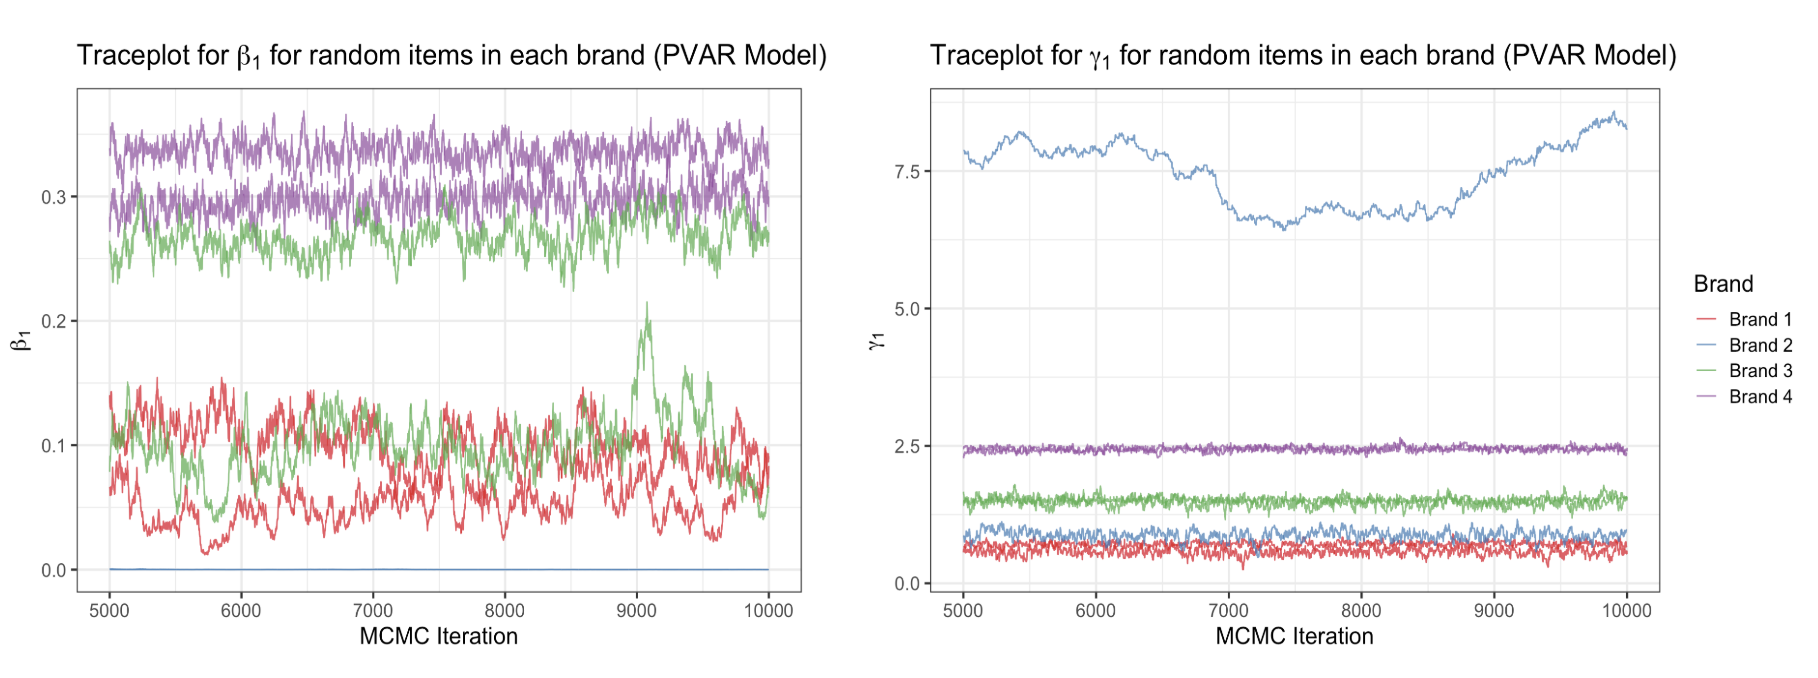
\includegraphics[width=1\linewidth]{figures/traceplot_pvar.png}
    \caption{Traceplots for item-level AR-1 terms and promotion effect terms using the single-item PAR model.}
    \label{fig:traceplot_pvar}
\end{figure}


\subsection{Choice of Lag for PAR and PVAR Models}

\noindent We did explore some alternative choices of lag for the PAR and PVAR models. The downstream forecasting performance using lags $1$, $5$, and $10$ are summarized in Table \ref{tab:forecast-summary}. Performance metrics were first evaluated on each item, then we computed the mean and median metrics across all $118$ items in the dataset, which are presented in the table. We find that that for some outlier items, the PAR(1) model produces forecasts which are highly unrealistic, leading to highly inflated means. Comparing the mean evaluation metrics, we see justification of lag $5$ for both the PAR and PVAR models, which is the choice we used for the current analysis. However, we also observe that higher las (i.e. lag 10) for the PVAR model may be more suitable for $H$-step forecasting on the test set.


\begin{table}[ht]
\centering
\caption{Summary of Forecast Performance (Mean / Median across Items)}
\begin{tabular}{lcccc}
\toprule
Model & 1-step MSE & H-step MSE & 1-step Deviance & H-step Deviance \\
\midrule
PAR(1) & $3.989 \times 10^{15}$ / 7.868 & $1.197 \times 10^{20}$ / 9.416 & $3.542 \times 10^{9}$ / 757.3 & $6.265 \times 10^{11}$ / 834.9 \\
PVAR(1) & 24.78 / 7.694 & 29.84 / 8.001 & 941.3 / 759.3 & 1049.8 / 792.2 \\
PAR(5) & 25.21 / 7.489 & 30.51 / 7.923 & 940.2 / 748.2 & 1127 / 780.9 \\
PVAR(5) & 24.54 / 7.648 & 30.17 / 7.953 & 932.0 / 750.8 & 1052.0 / 786.2 \\
PAR(10) & 25.94 / 7.725 & 30.19 / 7.981 & 955.4 / 765.4 & 1077 / 820.9 \\
PVAR(10) & 26.46 / 7.994 & 29.95 / 7.972 & 963.2 / 758.0 & 1043.7 / 771.2 \\
\bottomrule
\end{tabular}
\label{tab:forecast-summary}
\end{table}
\end{document}
